\section{Resultados}

Uno de los objetivos de la experimentación de este trabajo era encontrar los mejores parámetros para los métodos, es decir, los parámetros para los cuales los algoritmos proporcionaban mejores resultados. Para determinar la calidad de los resultados obtenidos (cuáles eran los mejores) se tuvo en cuenta distintas métricas, que ayudaron a determinar esto mismo:

\begin{itemize}
\item Accuracy
\item F1-Score
\end{itemize}

Los resultados obtenidos fueron analizados en términos de estas métricas aplicando validación cruzada \textit{K-fold}, variando el $K$ sobre la base de entrenamiento.

Los parámetros $k$ (cantidad de vecinos en \textit{kNN}, no confundir con $K$ de \textit{K-fold}) y $\alpha$ (dimensión a la cual se reduce cada imagen con \textit{PCA}) fueron variándose como se expondrá en las páginas siguientes.

Además de las métricas mencionadas, se tuvo en cuenta el tiempo de computo para las distintas entradas.

\subsection{Tiempo de ejecución kNN}

Dado que el costo temporal de kNN no depende del parámetro k, lo que nos interesa es entender el costo fijo por predicción. En un dataset de 205 imágenes reducidas, el costo promedio de clasificación de una imágen fue de 0.00042. Comparamos ese resultado con el costo promedio para la misma cantidad de imágenes de tamaño completo y el resultado fue 0.11738, varios órdenes de magnitud mayor. 

\subsection{Tiempo de ejecución PCA+kNN}

Para evaluar el costo temporal de las predicciones de kNN al utilizar PCA, es necesario tener en cuenta el costo de la transformación característica (tc), que se realiza a cada imágen a predecir para poder compararla con las imágenes de entrenamiento transformadas gracias al PCA. Otro factor a tener en cuenta es que el $\alpha$ de PCA define la dimensión de las imágenes que compara el kNN, esto impacta directamente a la cantidad de operaciones necesarias y consecuentemente al tiempo de cómputo.

\begin{figure}[H]
	\begin{center}
      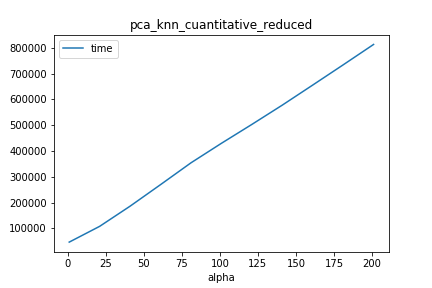
\includegraphics[width=0.4\columnwidth]{imagenes/charuli-des/pca_knn_cuantitative_reduced.png}
      \caption{Costo temporal de tc + predicción de kNN}
      \end{center}
\end{figure}

\subsection{Tiempo de ejecución PCA}

Con el objetivo de entender el costo de calcular una matriz de covarianzas para una muestra X, probamos con diferentes cantidades de imagenes reducidas y con diferentes valores del alfa de PCA. 

Para visualizar los resultados de los experimentos para cada X, se creó un gráfico donde la variable independiente es el alpha y la variable dependiente es el tiempo de cómputo. 

En los gráficos Observamos que el tiempo de cómputo se comporta de forma lineal en ralción al alpha para distintos segmentos de alpha, pero la pendiente es discontinua. No se pudo encontrar una causa evidente a esta falta de continuidad.//
Notar que el método descrípto en la sección $Desarrollo$ para obtener la matríz de covarianzas $M$ a partír de $\^{M}$, no pudo ser implementado completamente. Se estima que éste método reduciría significativamente el cálculo de la matríz de covarianza M (que es lo que más tiempo consume de todo el programa). 

\begin{figure}[H]
	\begin{center}
      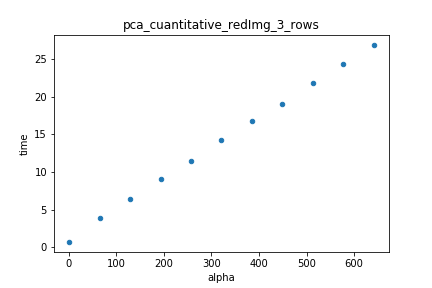
\includegraphics[width=0.4\columnwidth]{imagenes/charuli-des/pca_cuantitative_redImg_3_rows.png}
      \caption{Costo temporal de PCA para tres imágenes reducidas}
      \end{center}
\end{figure}
\begin{figure}
	\begin{center}
    	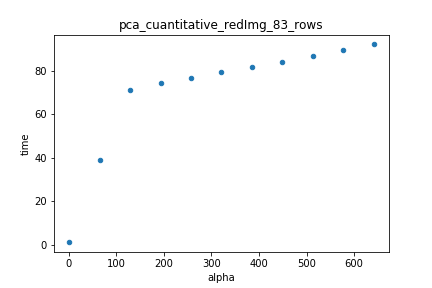
\includegraphics[width=0.4\columnwidth]{imagenes/charuli-des/pca_cuantitative_redImg_83_rows.png}
     \caption{Costo temporal de PCA para ochenta y tres imágenes reducidas}
     \end{center}
\end{figure}

\subsection{K de kNN}
 
Utilizamos las imagenes de tamaño completo, sin transformaciones. Llamamos k a la constante que define cuantos vecinos se tienen en cuenta a la hora de decidir la categoría de la muestra a clasificar. Los valores probados para k fueron 1, 3, 8, 10, 15 y 25. Se observó consistentemente que todas las métricas decrecen a medida que se incrementa el valor de k. Siendo $k = 1$ el valor óptimo.
 
\begin{figure}[H]
    \begin{center}
      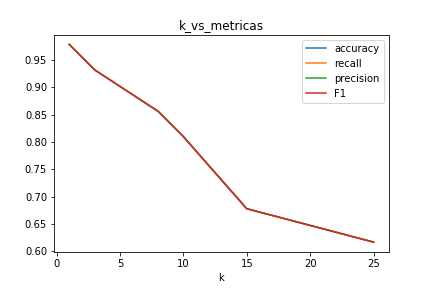
\includegraphics[width=0.6\columnwidth]{imagenes/charuli-des/k_vs_metricas.png}
      \caption{Metricas para distintos valores de k}
    \end{center}
\end{figure}
 
La diferencia en la calidad de las predicciones tambien puede observarse  visualizando matrices de confusión.
 
\begin{figure}[H]
    \begin{center}
      \includegraphics[width=0.6\columnwidth]{imagenes/charuli-des/Confusion_matrix_for_k_1.png}
      \caption{Metricas para distintos valores de k}
    \end{center}
\end{figure}
 
\begin{figure}[H]
    \begin{center}
      \includegraphics[width=0.6\columnwidth]{imagenes/charuli-des/Confusion_matrix_for_k_25.png}
      \caption{Metricas para distintos valores de k}
    \end{center}
\end{figure}
 
El mejor puntaje obtenido utilizando kNN con k=1 fue accuracy: 0.978049  recall: 0.978049  precision: 0.978049  F1: 0.978049
 
\subsection{Calidad al usar PCA }
 
Al utilizar PCA y kNN tenemos dos parámetros con los cuales experimentar. Se probaron combinaciones entre los k de kNN 1, 3, 8, 10, 15, 25 y los alpha de PCA 3, 10, 25, 40, 60.
 
Para estudiar el comportamiento de K se realizo la operación groupby de pandas DataFrames (escencialmente lo mismo que un groupby de SQL) logrando que para cada valor diferente de k de promedien los valores de cada métrica independientemente del valor de alpha.  Puede observarse al igual que el uso kNN sin pca, los mejores resultados se obtienen mirando un solo vecino.
 
 
 
\begin{figure}[H]
    \begin{center}
      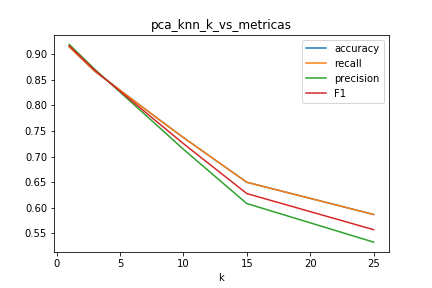
\includegraphics[width=0.6\columnwidth]{imagenes/charuli-des/pca_knn_k_vs_metricas.png}
      \caption{k vs metricas, con alpha promediado}
    \end{center}
\end{figure}
 
Puede observarse la diferencia entre dos matrices de confusión.
 
\begin{figure}[H]
    \begin{center}
      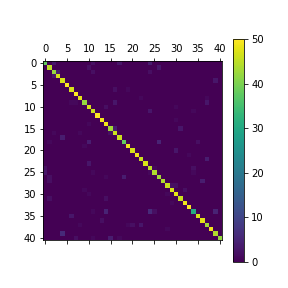
\includegraphics[width=0.6\columnwidth]{imagenes/charuli-des/pca_knn_confusion_matrix_for_k_1.png}
      \caption{Matriz de confusion para k=1, alpha promediado}
    \end{center}
\end{figure}
 
\begin{figure}[H]
    \begin{center}
      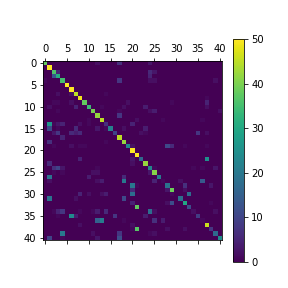
\includegraphics[width=0.6\columnwidth]{imagenes/charuli-des/pca_knn_confusion_matrix_for_k_25.png}
      \caption{Matriz de confusion para k=25, alpha promediado}
    \end{center}
\end{figure}
 
 
Para estudiar el comportamiento de alpha se realizó el mismo procedimiento invirtiendo los roles de ambos parámetros. Se puede observar que las métricas mejoran a medida que aumenta alpha,  pero cada vez menos.
\begin{figure}[H]
    \begin{center}
      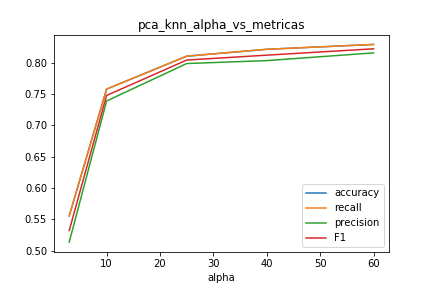
\includegraphics[width=0.6\columnwidth]{imagenes/charuli-des/pca_knn_alpha_vs_metricas.png}
      \caption{alpha vs metricas, con k promediado}
    \end{center}
\end{figure}
 
Puede observarse la diferencia entre dos matrices de confusión.
 
\begin{figure}[H]
    \begin{center}
      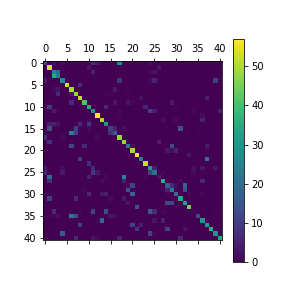
\includegraphics[width=0.6\columnwidth]{imagenes/charuli-des/pca_knn_confusion_matrix_for_alpha_3.png}
      \caption{Matriz de confusion para alpha=3, k promediado}
    \end{center}
\end{figure}
 
\begin{figure}[H]
    \begin{center}
      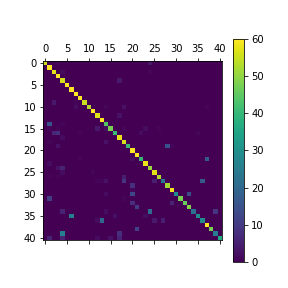
\includegraphics[width=0.6\columnwidth]{imagenes/charuli-des/pca_knn_confusion_matrix_for_alpha_60.png}
      \caption{Matriz de confusion para alpha=60, k promediado}
    \end{center}
\end{figure}
 
 
Se pueden visualizar ambos efectos utilizando un gráfico de dispersión, en el cual los mejores puntajes son representados por puntos fucsias, cercanos a uno y los peores representados por puntos celestes, cercanos a cero.
\begin{figure}[H]
    \begin{center}
      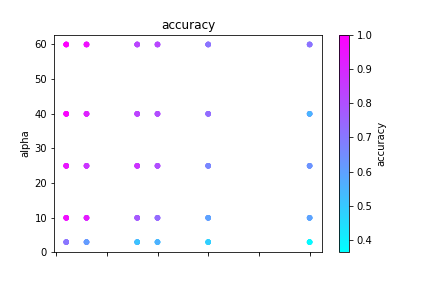
\includegraphics[width=0.6\columnwidth]{imagenes/charuli-des/k_and_alpha_vs_accuracy.png}
      \caption{alpha y k vs metricas}
    \end{center}
\end{figure}
 
 
El mejor puntaje obtenido utilizando kNN y PCA con k=1 y alpha=60 fue accuracy: 0.978049  recall: 0.978049  precision: 0.979675  F1: 0.978853
